%!TEX root = main.tex

\subsubsection{\stid{1.04} SNL ATDM Programming Models: DARMA} 

\paragraph{Overview} 
DARMA (Distributed, Asynchronous, Resilient Models for Applications) embeds safe and performant asynchronous tasking constructs in C++.
DARMA defines asynchronous semantics for C++, providing a futures-based programming model. 
DARMA, however, provides additional semantics that carry extra safety and performance guarantees,
including race freedom, fully non-blocking execution, and simplified load balancing and communication overlap.
These semantics are implemented as a standards-compliant C++ header library,
embedding asynchronous execution via metaprogramming.

\paragraph{Key Challenges}
Dynamic applications can be characterized by either unknown, imbalanced, or rapidly varying computation loads and communication patterns.
Particle-in-cell, for example, has varying computational load per mesh region. As particles migrate, it also requires dynamic termination detection before entering a field solve phase. 
Overlap detection in contact algorithms rapidly creates load imbalance, which must be mitigated dynamically, in regions where contact occurs. Addressing these algorithmic challenges can involve:
\begin{itemize}
\item Latency-hiding of communication by trying to improve overlap with computation
\item Elastic tasks with built-in data parallelism that can leverage more cores for larger tasks
\item Asynchronous quiescence detection to avoid global synchronizations and minimize communication
\item Semi-static load balancing (globally synchronous) for problems with persistent load imbalance
\item Dynamic load balancing (work stealing) for problems with rapidly varying load imbalance
\end{itemize}
One possible option is for application developers to pursue domain-specific, ad hoc solutions.
Managing things like resource contention between elastic tasks or implementing spanning trees for quiescence are highly non-trivial.
A far more sustainable and productive approach would be providing these execution patterns in a reusable library with implementation complexities hidden behind a productive programming model.
Programming should emphasize problem decomposition, data effect specification for correctness, and domain-specific cost models and heuristics for performance portability.
The key challenges are both defining the programming abstractions to be used at application-level and implementing these dynamic execution constructs at the runtime-level.

\paragraph{Solution Strategy}
Similar to standard futures that create data-flow for C++ datatypes,
DARMA provides asynchronous pointers with well-defined semantics that augment data-flow with non-blocking and race freedom guarantees.
DARMA asynchronous pointers cab define serialization for arbitrary C++ types, enabling load balancing and asynchronous communication overlap.
DARMA asynchronous pointers are intended to express concurrency in a sufficiently general way that multiple runtimes could serve as the backend implementation (Figure~\ref{fig:darmaStack}).
To date, HPX (futures/promises), Charm++ (actor model), and MPI + OpenMP have all been able to provide relatively lightweight implementations despite their obvious design differences.


\begin{figure}
\centering
\includegraphics[width=0.5\textwidth]{projects/2.3.1-PMR/2.3.1.04-SNL-ATDM-PMR/DARMA_Software_Stack.pdf}
\caption{DARMA software stack model showing application-level code implemented with asynchronous programming model (DARMA header library).
Application-level semantics are translated into a task graph specification via metaprogramming in the translation layer. Glue code maps task graph specification to individual runtime libraries. Current backend implementations include std::threads, Charm++, MPI + OpenMP, and HPX.}
\label{fig:darmaStack}
\end{figure}
%\end{minipage}

%\begin{minipage}{0.5\textwidth}
%\begin{figure}
%\includegraphics[width=0.9\textwidth]{DARMA_Software_Stack.pdf}
%\end{figure}
%\end{minipage}

Another general approach consistent with the DARMA model for reducing algorithmic complexity is task \emph{over-decomposition} in the context of shared-memory parallelism.
For example, taking an MPI rank as the fundamental unit, over-decomposition would create many (e.g. 4-16) regions or patches per MPI rank,
rather than a single large patch as would be most common.
Overdecomposition aims to avoid complexities in explicit, application-level load balancing and explicit, application-level communication latency hiding.
When load imbalance occurs, entire tasks can be migrated without requiring re-meshing or updating data structures.
Similarly, communication occurs transparently through task dependencies, naturally pipelining and overlapping communication without requiring explicit Isend/wait constructs.

DARMA allows algorithms to be expressed with flexible granularity, tuning overdecomposition factors to meet either a hardware requirement (e.g. optimal balance of communication overlap and scheduling overhead, task blocking to fit caches) or an algorithmic requirement (e.g. sufficiently fine granularity for load balancing).
Recent DARMA-Kokkos integration now allows over-decomposition on a per-node basis, rather than per-core.
This greatly minimizes task scheduling overheads and can improve communication throughput (surface area-to-volume considerations).
This further improves load balancing flexibility by allowing DARMA to control not only the number of tasks per node but the number of cores allocated to each task.

\paragraph{Recent Progress}
DARMA constructs are being used in the development of ATDM applications, including particle-in-cell (as part of EMPIRE), multiscale physics (in the ATDM tech demonstrator), and contact applications.  MPI interoperability constructs have been defined and recently implemented. DARMA has integrated with Kokkos, providing support for data-parallel tasks.

\paragraph{Next Steps}
The next steps are pursuing both continued adoption in further applications, continued implementation of the programming model with additional backends, and continued improvement of the MPI + OpenMP reference implementation.
For application adoption, a major focus will be using the MPI interoperability constructs to interface Trilinos solvers with DARMA kernels.
Code improvements of the MPI reference implementation will focus on more load balancing heuristics, performance and correctness debugging, and demonstration at increasing scales on capability platforms like Trinity, Cori, and Sierra.
DARMA is also active on the C++ standards committee, particularly for the parallelism technical specification. DARMA-inspired library features are being actively proposed and considered.